\chapter{Dealing with geographical variation: hepatitis C virus infection}
\label{applications-rfx}
\chapterprecis{Abraham D. Flaxman, Khayriyyah M. Hanafiah, Justina Groeger, Hannah M. Peterson, and Steven T. Wiersma}

One challenge in global disease modeling for descriptive
epidemiological estimation is properly reflecting the true regional
variation in disease epidemiology. While some diseases are relatively
consistent in their levels and age patterns from region to region,
others vary a great deal.  The most extreme examples of the latter type are focal
diseases that are present only in certain regions, but the hardest to
model are diseases that are present globally, but to greater and lesser
degree.  Hepatitis C virus (HCV) is an example of such a disease,
which we examine in this chapter.  In the absence of any strongly
predictive covariates, we use hierarchical random effects to model
this regional variation.

Hepatitis C is a disease caused by the viral infection of HCV, an RNA
virus in the Flaviviridae family that
predominately attacks the liver.  In a small
portion of acute cases, the body can eliminate the virus; however, the
majority of acute cases develop into chronic infections.  Chronic
infections cause liver damage and may develop into end-stage liver
disease, or cirrhosis.  Few of those persons who are chronically infected experience symptoms,
and only one-third of acute cases develop jaundice or other symptoms.
Chronic symptoms are nonspecific, intermittent, and mild, with the most
common symptom being fatigue.  Common symptoms for severe and advanced
disease stages include nausea, dark urine, and jaundice.  Since
HCV infections are often asymptomatic, diagnosis usually requires laboratory
testing for both hepatitis antibodies (anti-HCV) which, when positive, indicates past or current infection and the HCV nucleic acid
(HCV RNA) which, when positive, indicated current infection.
There is no vaccine that protects against HCV infection, but
new treatments have been reported to clear the infection and
prevent advanced liver disease.\cite{hoofnagle_hepatitis_1997, ghany_diagnosis_2009, ghany_update_2011}

Compared with other countries in the North Africa / Middle East region,
Egypt has a high prevalence of HCV infection in the general population.  In an attempt to treat
endemic schistosomiasis, a common parasitic worm that affects the
urinary tract, gut, and liver, the Egyptian Ministry of Health launched
widespread injection-based treatment from 1950 to 1980.  While
there were improvements in schistosomiasis-induced mortality, recycled
needles and poor needle sterilization used to deliver these medicines inadvertently infected many with HCV.
\cite{frank_role_2000, mezban_hepatitis_2006, strickland_liver_2006}
The spatial variations of HCV infection in
North Africa and the Middle East provides a striking example for
hierarchical random-effects modeling.

Random-effects modeling detects systematic differences among different
spatial units of data.  The spatial hierarchy in the GBD
2010 Study uses countries nested in regions nested in superregions.
There are $21$ regions defined by demographic and epidemiological
similarities, which are further clustered into $7$ superregions (see appendix~\ref{appendix-hierarchy}).

The analysis of HCV infection uses data on the prevalence of persons who
have antibodies to HCV (anti-HCV).  Incomplete data or data from high-risk
populations, such as injection drug users or paid blood donors, were excluded.
Figure~\ref{fig:app-hepc data} shows data collected in systematic
review for two countries in the North Africa / Middle East region, Egypt
and Jordan.  Notice that for some age groups, anti-HCV prevalence
measurements in Egypt are more than $40$ times higher than the corresponding measurements in
Jordan.

    \begin{figure}[h]
        \begin{center}
            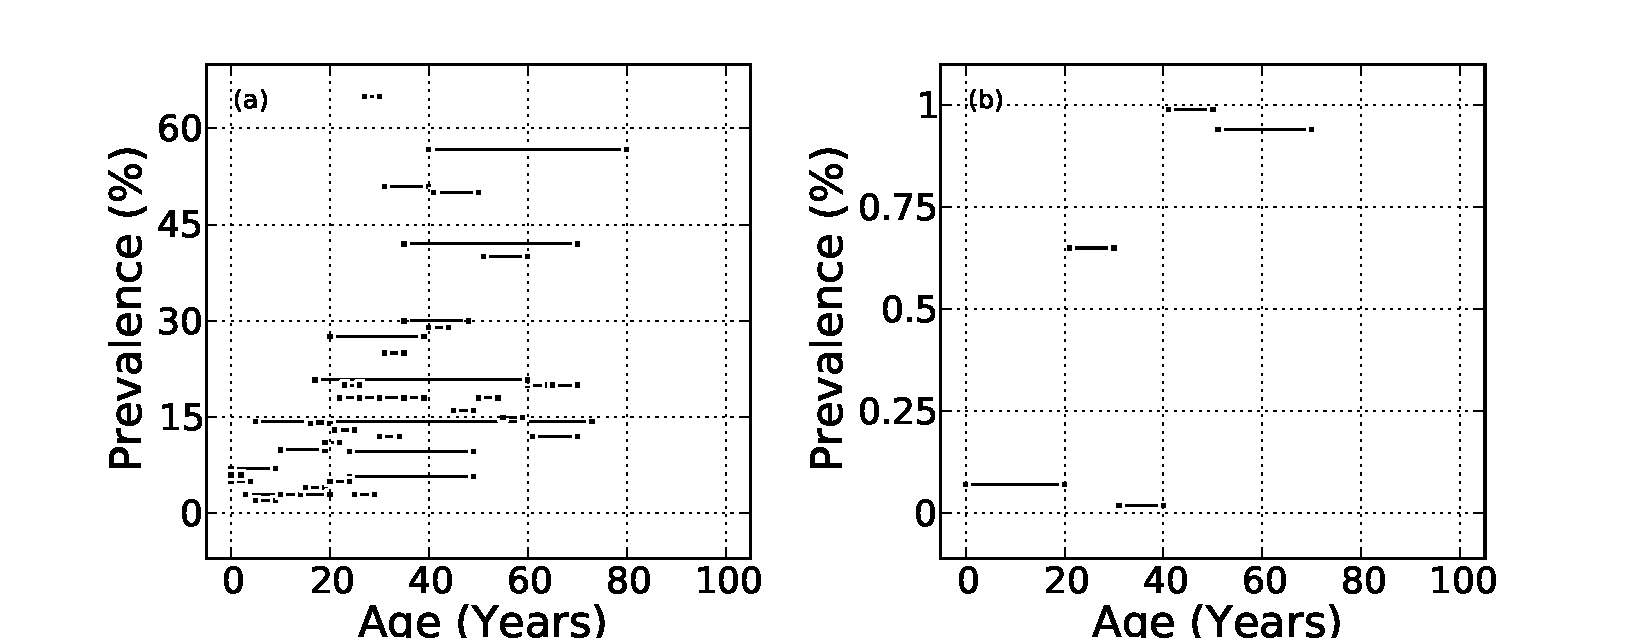
\includegraphics[width=\textwidth]{hepc-EGY_v_JOR.pdf}
            \caption{Prevalence data from systematic review of
              anti-HCV in (a) Egypt and (b) Jordan.}
            \label{fig:app-hepc data}
        \end{center}
    \end{figure}

We used the age-standardizing, generalized negative-binomial spline
model with hierarchical random effects to estimate anti-HCV prevalence.  The
hierarchical random effects allow the model to capture variation
within the North Africa / Middle East region.
Table~\ref{tab:app-hepc regional rfx} shows that Egypt has significantly
higher prevalence than the other countries in the region.
Figure~\ref{fig:app-hepc regional rfx} confirms this, as the prevalence
estimate for Egypt is much above the regional average.

    \begin{table}[h]
        \caption[Estimates of the country-level random effects for anti-HCV
          prevalence]{Estimates of the country-level random effects for anti-HCV
          prevalence (an intercept shift in log-space) from the random-effects
          model for the countries in the North Africa / Middle
          East region}
        \label{tab:app-hepc regional rfx}
        \begin{center}
        \begin{tabular}{|c|c|c|c|}
            \hline
                Country & Posterior Mean & Lower 95\% HPD  & Upper 95\%  HPD \\
            \hline
                Egypt	&	1.87	&	 1.5	&	2.2	\\
                Jordan	&	-0.59	&	-1.1	&	-0.1 \\
                Saudi Arabia	&	-0.77	&	-1.2	&	-0.4 \\
                Iraq	&	0.07	&	-0.4	&	0.6	\\
                Iran	&	0.02	&	-0.4	&	0.5	\\
                Yemen	&	0.04	&	-0.4	&	0.4	\\
                Turkey	&	-0.31	&	-0.7	&	0.0	\\
                Syria	&	-0.13	&	-0.7	&	0.4	\\
                Tunisia	&	-0.19	&	-0.7	&	0.3	\\
            \hline
        \end{tabular}
        \end{center}
    \end{table}

    \begin{figure}[h]
        \begin{center}
            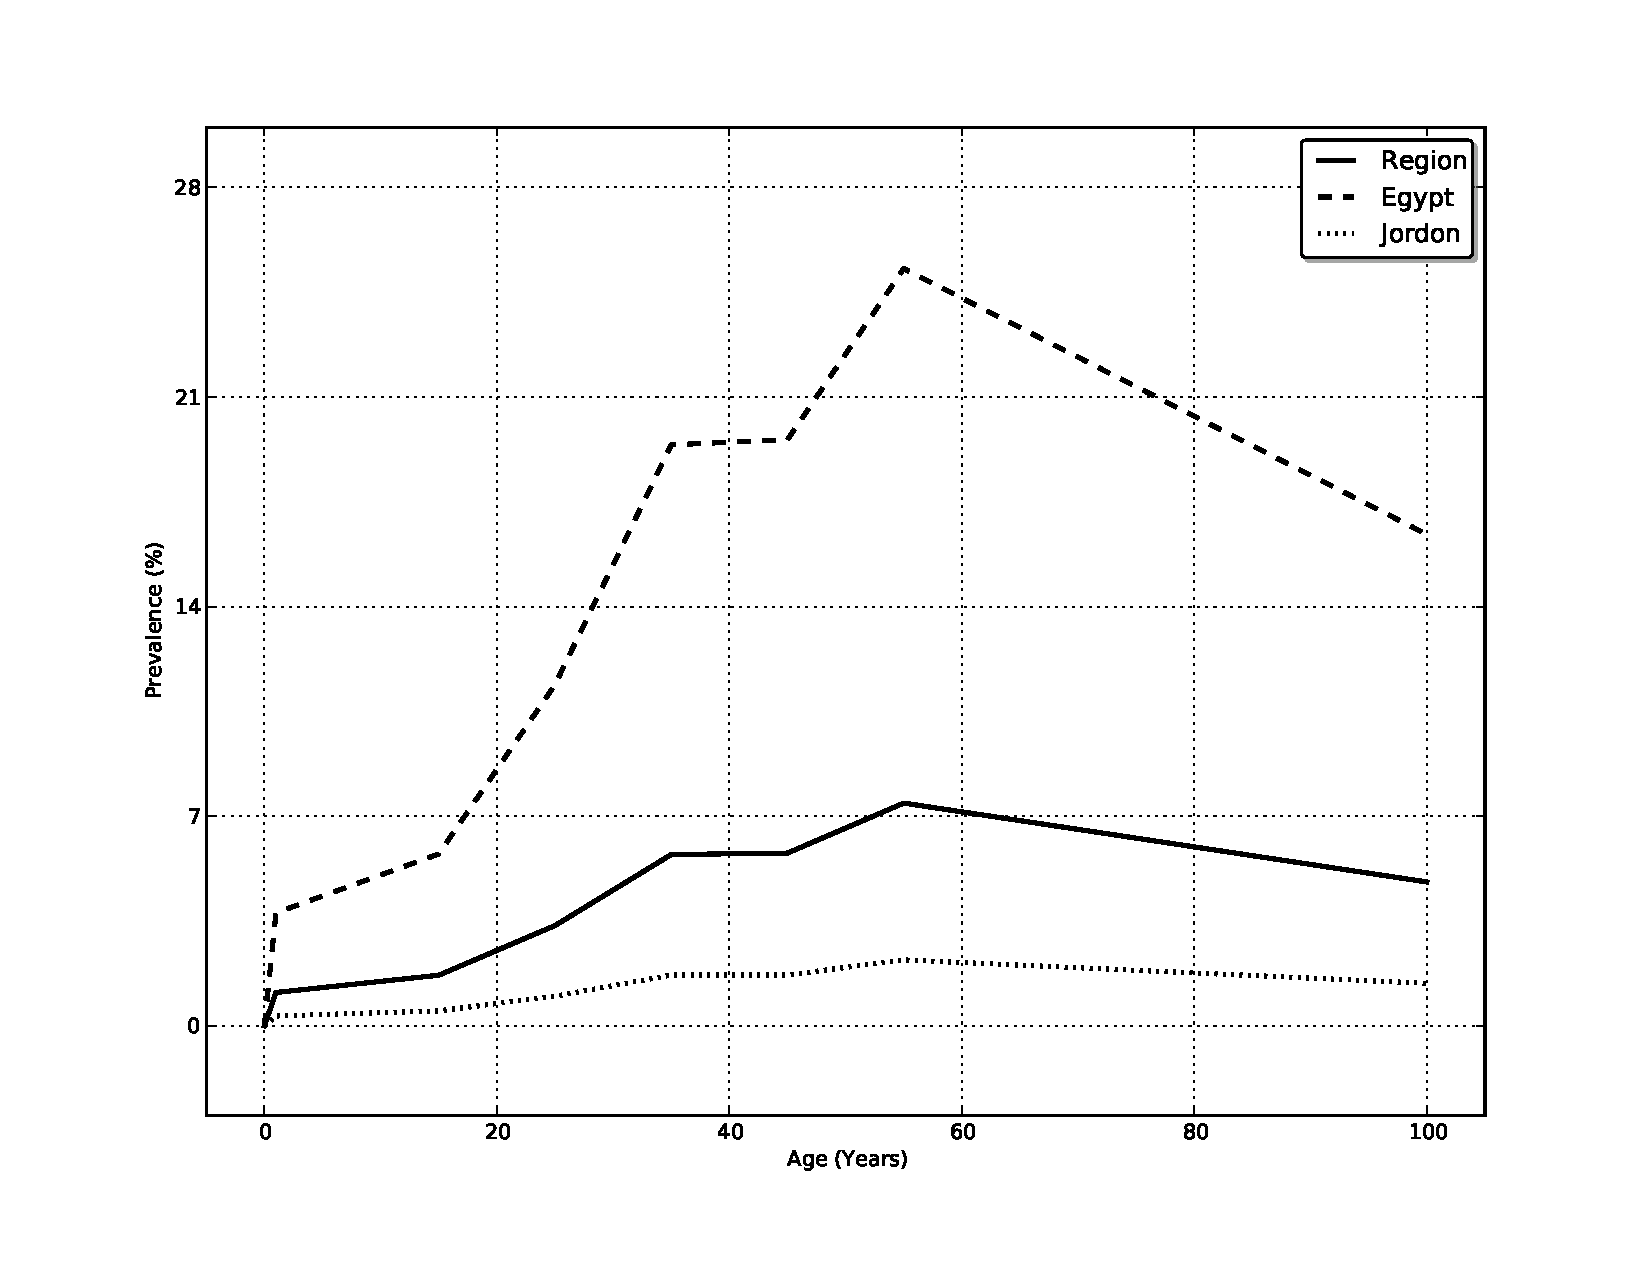
\includegraphics[width=\textwidth]{hepc-region_v_EGY_v_JOR.pdf}
            \caption[Estimates of anti-HCV prevalence in North Africa / Middle East 
              region and in the countries Egypt and Jordan.]{The 1990 estimate of 
              anti-HCV prevalence for
              men in the North Africa / Middle East region and in
              the countries Egypt and Jordan.  These estimates
              use only $2$ levels in the hierarchical random-effects
              model: region and country.}
            \label{fig:app-hepc regional rfx}
        \end{center}
    \end{figure}

In addition to hierarchical random effects, the negative-binomial
rate model includes a parameter that estimates
the amount of nonsampling error, parametrized as the overdispersion
term $\delta$, described in chapter~\ref{theory-rate_model}.
In such noisy data, weakly informative priors on $\delta$ help with
convergence and inform the posterior estimates about beliefs
regarding data heterogeneity.  This allows the model to incorporate
expert beliefs about how much of the country-to-country variation is
true variation and how much is nonsampling error, which can be
important in the presence of sparse and noisy data.  We compared three
alternative priors on the negative-binomial model dispersion
parameter $\delta$, corresponding to ``very,'' ``moderately,'' or
``slightly'' overdispersed.  The natural logarithm of $\delta$ is
uniformly distributed between its lower and upper bounds.  Intended as
a weakly informative prior, the bounds of the categories of $\delta$ overlap, so
that the bounds of ``very,'' ``moderately,'' and ``slightly'' are $[1,9]$, $[3,27]$, and
$[9,81]$, respectively.

In this example, the effects of priors on the overdispersion of
$\delta$ are seen in the posterior estimates at the country level as
shown in figure~\ref{fig:app-hepc global hetero}.  Random-effects
modeling detects within-sample variation and true variation that
cannot be explained by a covariate.  Therefore, a change in the prior
on global heterogeneity changes the level of variation and thus the
size of the random effect.  As seen in figure~\ref{fig:app-hepc global
  hetero}, when the prior on overdispersion is ``very,'' the estimates
are more compressed than those with a prior of ``slightly.''

    \begin{figure}[h]
        \begin{center}
            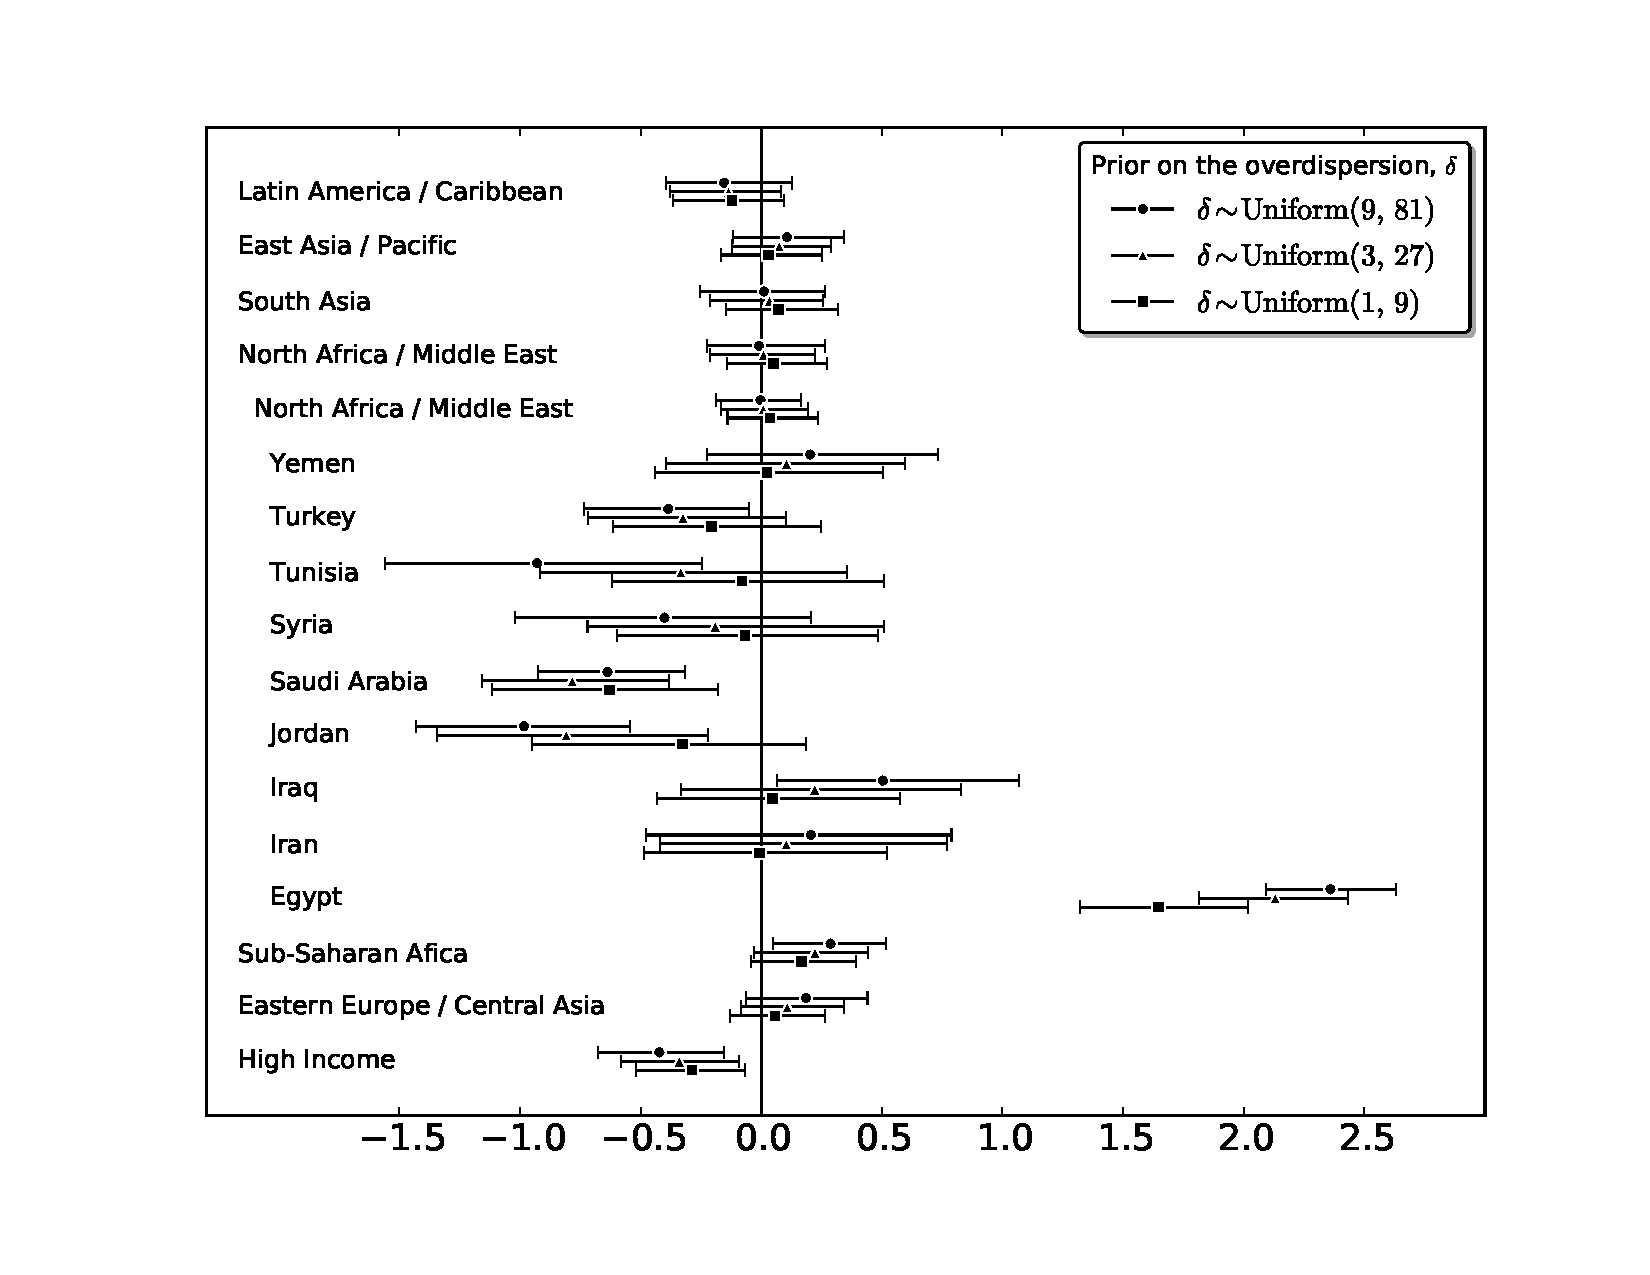
\includegraphics[width=\textwidth]{hepc-tree_plot_global_hetero.pdf}
            \caption[The intercept shift of anti-HCV
              prevalence with different priors on global heterogeneity.]{The intercept shift of anti-HCV
              prevalence for men in 1990 in log-space with different priors on
              global heterogeneity, $\delta$.  Four levels (global,
              superregion, region, country) were used in the
              hierarchical random-effects spline model.}
            \label{fig:app-hepc global hetero}
        \end{center}
    \end{figure}

Another way to view compressed estimates is by looking at the
age-standardized prevalence in table~\ref{tab:app-hepc global rfx}.
As heterogeneity increases from ``slightly'' to ``very,'' country
estimates are compressed toward the regional mean.

    \begin{table}[h]
        \caption{Anti-HCV age-standardized prevalence estimates
          from a hierarchical random-effects spline model with differing
          priors on global heterogeneity}
        \label{tab:app-hepc global rfx}
        \begin{center}
        \begin{tabular}{|c|c|c|c|}
            \hline
                & & Posterior & Standard \\
                Geographic Area & Heterogeneity & Mean & Deviation \\
            \hline
                & $\delta \sim \Uniform(9,81)$ & 0.048 & 0.003 \\
                North Africa/Middle East & $\delta \sim \Uniform(3,27)$ & 0.049 & 0.004 \\
                & $\delta \sim \Uniform(1,9)$ & 0.045 & 0.005 \\
            \hline
                & $\delta \sim \Uniform(9,81)$ & 0.007 & 0.002 \\
                Jordan & $\delta \sim \Uniform(3,27)$ & 0.010 & 0.003 \\
                & $\delta \sim \Uniform(1,9)$ & 0.020 & 0.007 \\
            \hline
                & $\delta \sim \Uniform(9,81)$ & 0.188 & 0.012 \\
                Egypt & $\delta \sim \Uniform(3,27)$ & 0.179 & 0.018 \\
                & $\delta \sim \Uniform(1,9)$ & 0.137 & 0.019 \\
            \hline
        \end{tabular}
        \end{center}
    \end{table}

Hierarchical random effects and the overdispersion parameter
$\delta$ allow the model to distinguish between true
country-to-country variation and nonsampling error.  Weakly
informative priors on $\delta$ incorporate the modeler's beliefs about
data heterogeneity, while the hierarchical random effects provide a way
to model regional variation.  When a predictive covariate is
available, it can be used instead of random effects to explain the
country-to-country variation (as
chapter~\ref{applications-efx_country_level} will demonstrate), but in
the absence of this, geographic random effects provide a mechanism to
model the level of unexplained but true variation between different
areas.

